\section{Test Case}
\label{sec:testCase}

\subsection{Plant Description}
For our analysis we have chosen a 3-unit plant site as shown in Fig.~\ref{fig:layout}. The chosen layout 
is not representative of any existing plant but it is simply fictitious.
From a topographical perspective, a large body of water is located in proximity of the NPP and it is 
employed as ultimate heat-sink for the plant.

\begin{figure}
    \centering
    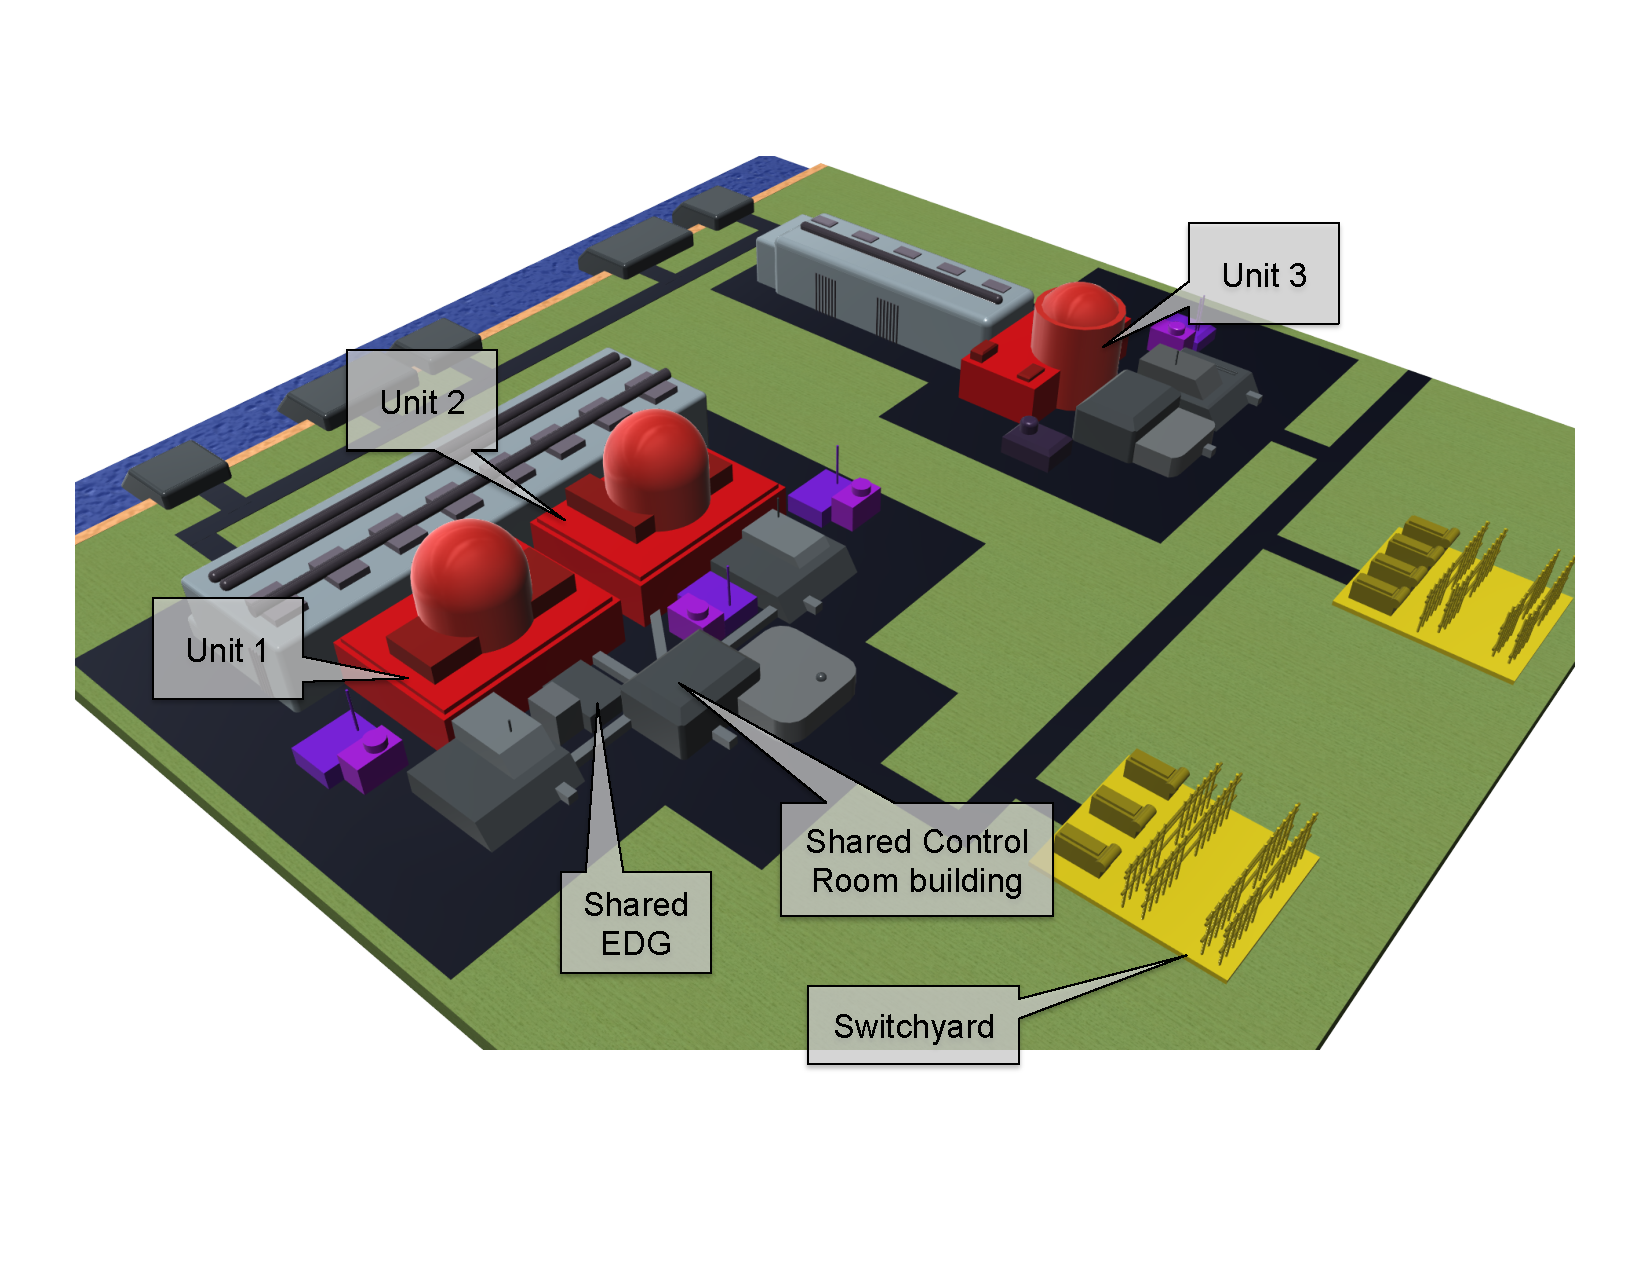
\includegraphics[scale=0.5]{layout.pdf}
    \caption{Overview of the multi-unit plant}
    \label{fig:layout}
\end{figure}

All three units are composed by Pressurized Water System (PWR) systems (see Fig.~\ref{fig:PWRscheme}); 
the design of the PWR systems are identical for all the three units and it 
can be considered generic, i.e., it is not specific to an existing plant. 

\begin{figure}
    \centering
    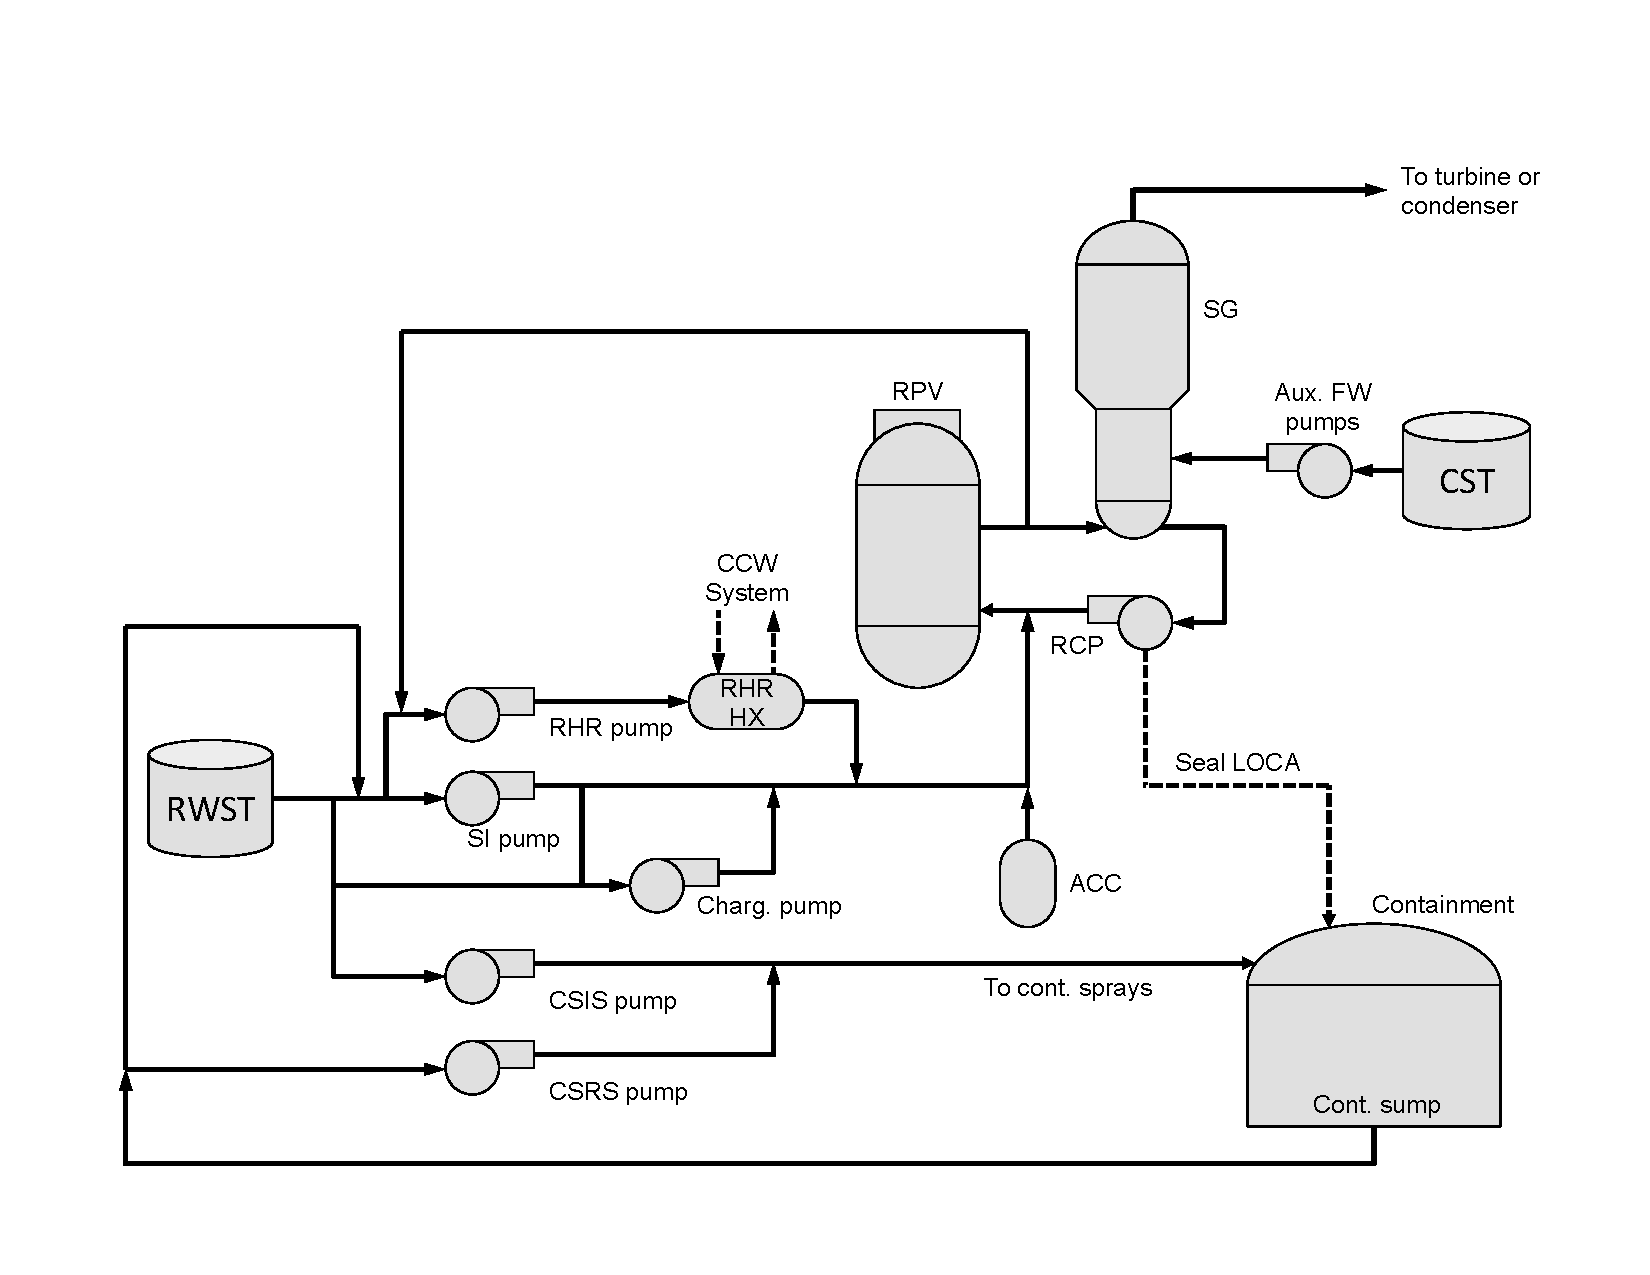
\includegraphics[scale=0.4]{PWRscheme.pdf}
    \caption{Generic scheme of a PWR system}
    \label{fig:PWRscheme}
\end{figure}

\begin{figure}
    \centering
    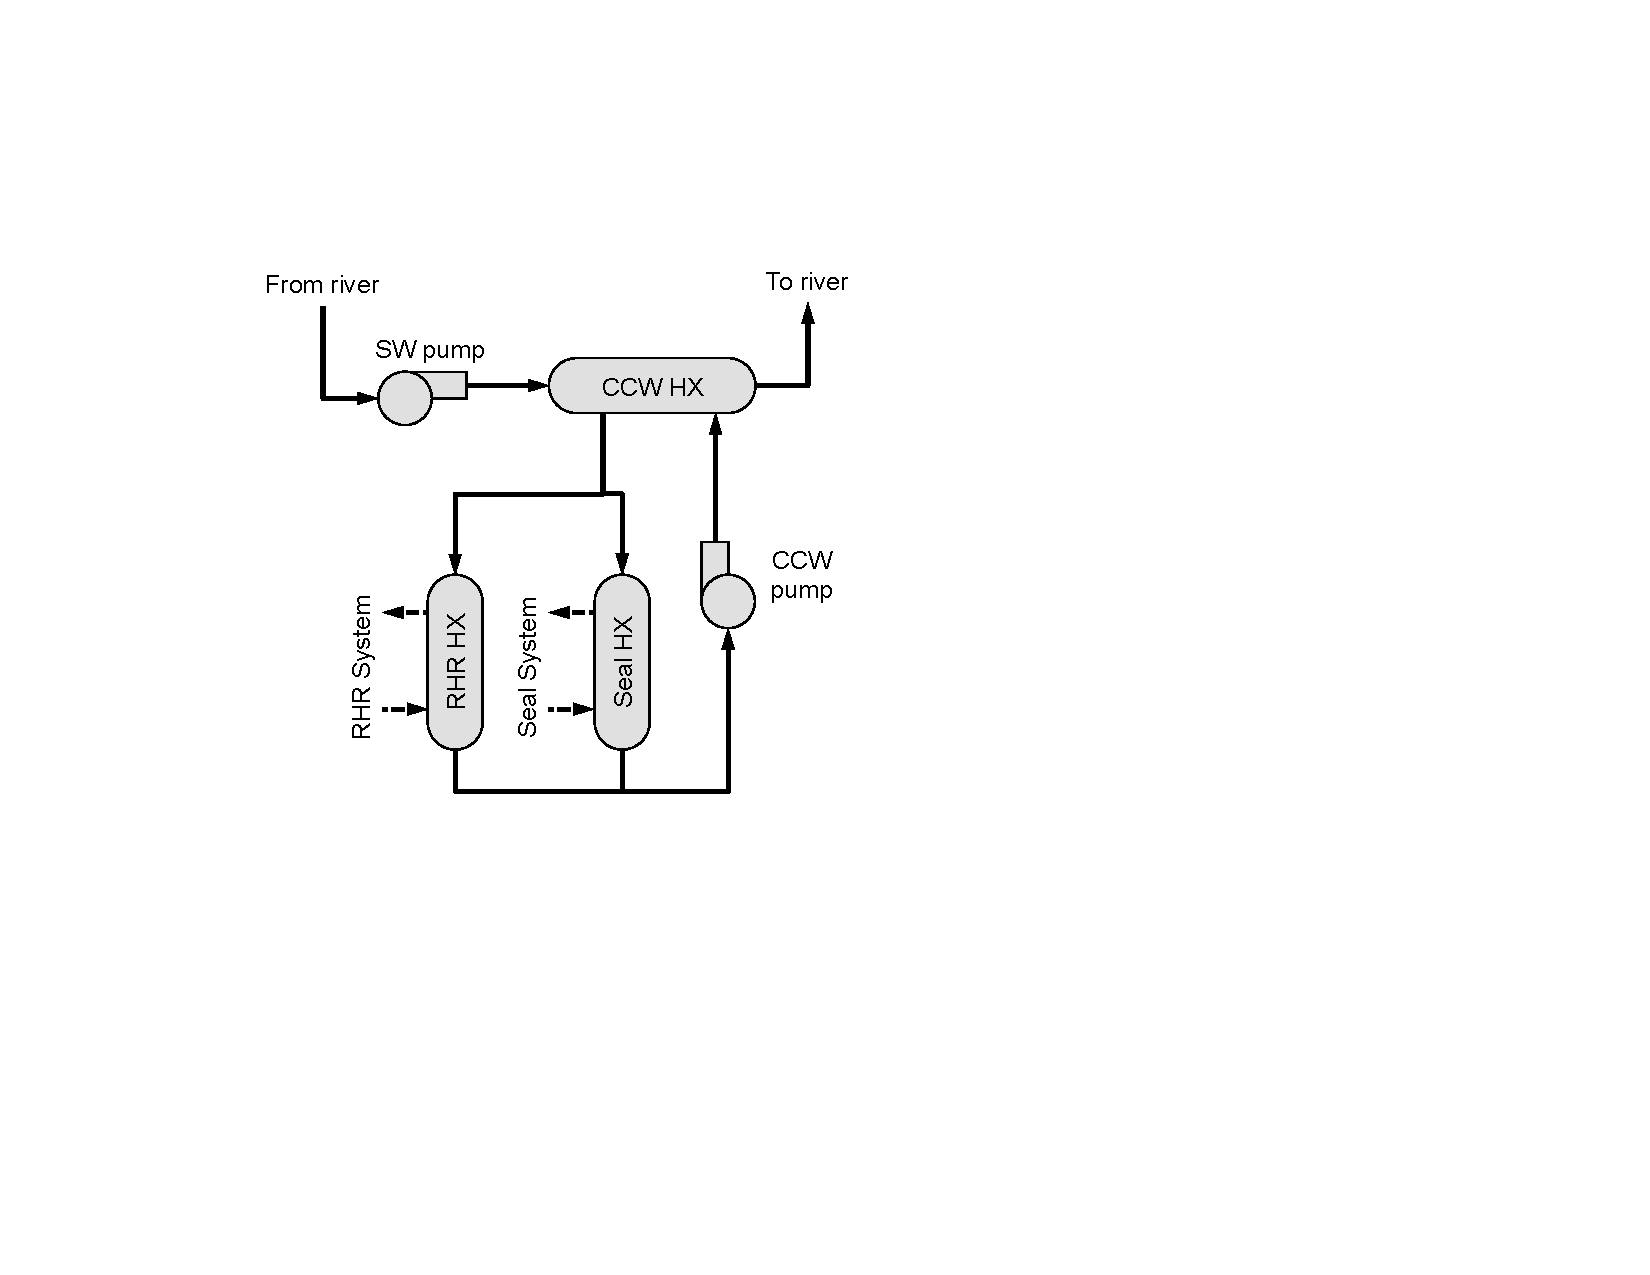
\includegraphics[scale=0.5]{CCW-SW.pdf}
    \caption{Generic scheme of a the CCW and SW systems}
    \label{fig:CCW-SWscheme}
\end{figure}

For each PWR, the systems considered in the analysis are the following:
\begin{itemize}
  \item High Pressure Injection System (HPIS)
  \item Low Pressure Injection System (LPIS)
  \item Residual Heat Removal (RHR) system
  \item Accumulators (ACCs)
  \item Auxiliary Feed-water (AFW) system 
  \item Charging pumps
\end{itemize}

Special attention has been given to the design of the electrical and hydraulic systems:
\begin{itemize}
  \item The plant electrical system is shown in Fig.~\ref{fig:electricalScheme}. Two 
        electrical switch-yards can provide electrical power to all units. All units 
        have a set of Emergency Diesel Generators (EDGs)  and, in addition, a swing 
        EDG (i.e., EDGS) can be employed to provide an alternate AC power to either
        Unit 1 or Unit 2. Note also that the 6.6 KV emergency buses of Unit 1 and 
        Unit 2 can be cross-tied.
  \item The AFW system of Unit 1 and Unit 3 can be cross-tied. 
        Thus cooling to the secondary side can be provided from one unit to the other one.
  \item The Condensate Storage Tanks (CSTs) of Units 2 and Unit 3 can be cross-tied. 
        Thus the water source  for the secondary side of either unit can be used as
        water source for the other one. 
  \item Plant recovery crew is a shared resource within the plant. In case of severe 
        accident scenarios, Emergency Portable Equipments (EPEs) can be employed in order
        to restore water flow or AC power into the PWRs or SFPs. Each unit has its own 
        set of EPEs but it is here assumed that a single EPE team (i.e., plant recovery 
        crew) is present within the plant boundaries.
\end{itemize}

\begin{figure}
    \centering
    \centerline{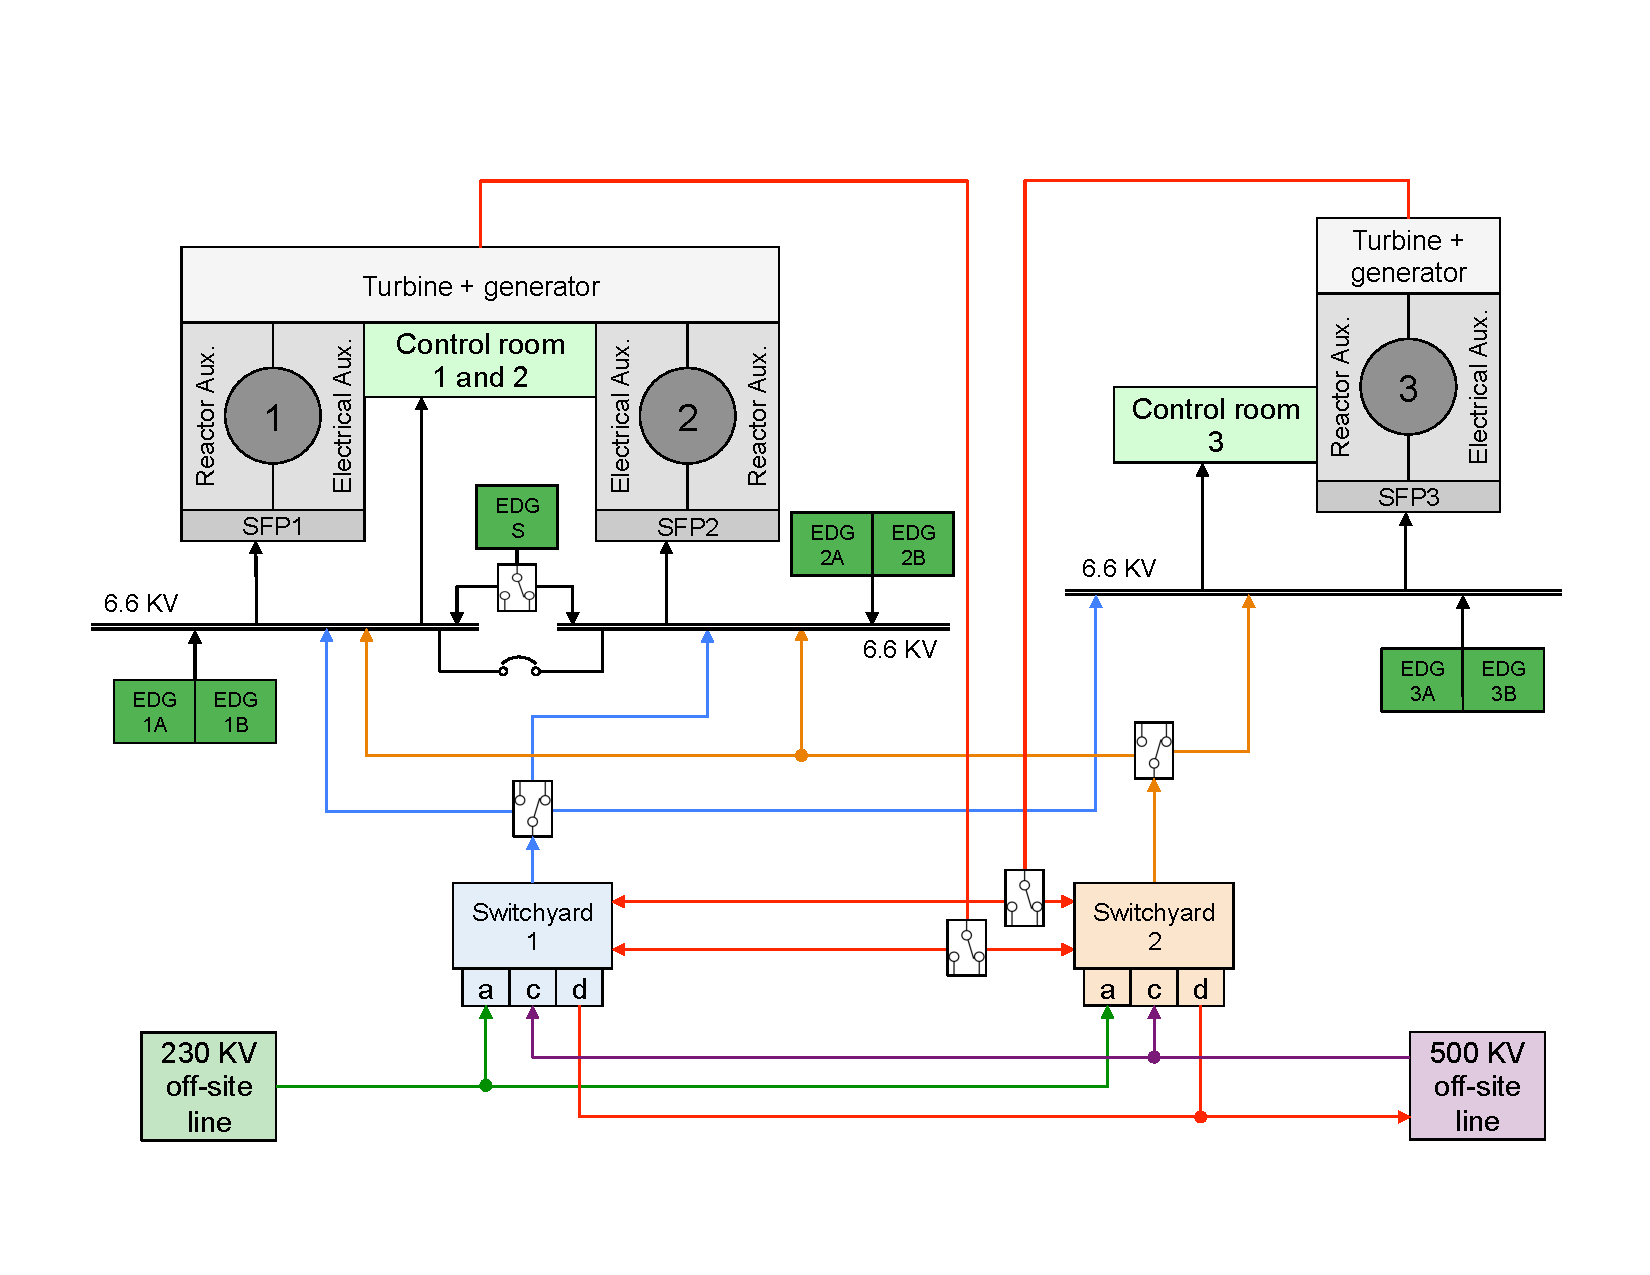
\includegraphics[scale=0.6]{electricalScheme.pdf}}
    \caption{Plant electrical scheme}
    \label{fig:electricalScheme}
\end{figure}

Figure~\ref{fig:schemeDep} summarizes the dependencies among the three units.

\begin{figure}
    \centering
    \centerline{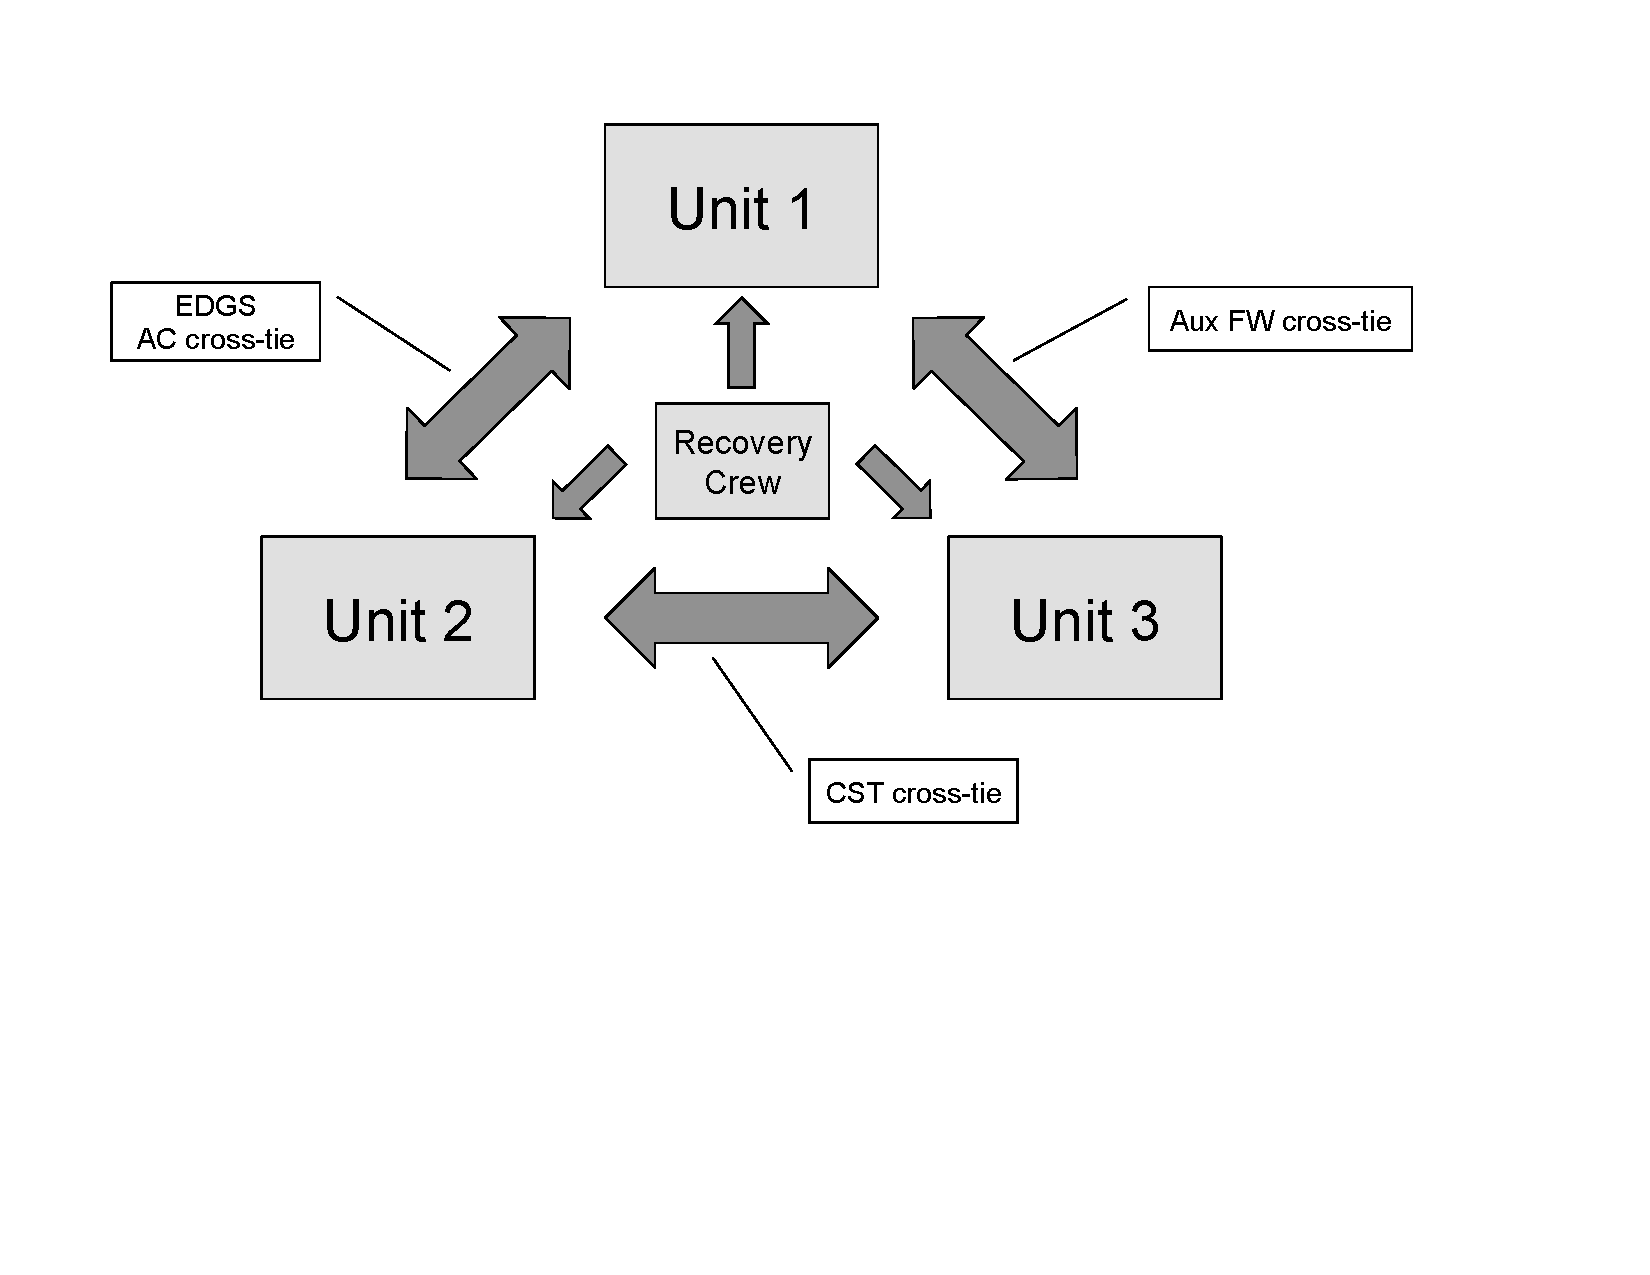
\includegraphics[scale=0.4]{schemeDep.pdf}}
    \caption{Summary of the dependencies among the three units}
    \label{fig:schemeDep}
\end{figure}

\subsection{Initiating Event}

The considered initiating event is a seismic event which causes the following events:
\begin{itemize}
  \item Both switch-yards are disabled
  \item All EDGs are disabled except EDGS which is operating and it is initially aligned to Unit 2
  \item CST of Unit 2 has lost 80\% of its capacity 
  \item CST of Unit 3 is completely lost
  \item The seismic event might also rupture the SFPs. Thus a leak might be present during the accident scenario
\end{itemize}

The proposed accident scenario resembles a Station Black Out (SBO) event at the plant level except for the 
fact that the EDGS is the only source of AC power available and it can be directed toward either Unit 1 or Unit 2.

Prior the seismic event, the three units initial conditions are summarized in Table~\ref{tab:unitsStatus}.

\begin{table}
  \begin{tabular}{ | l | p{10cm} | }
    \hline      
      \textbf{Unit} & \textbf{Initial Condition} \\
      \hline \hline
      1 &       The PWR of Unit 1 (i.e., PWR1) is at full power (100\% power level) and it own SFP \\ \hline
      2 &       The PWR of Unit 2 (i.e., PWR2) is in mid-loop operation (i.e., shut-down mode) and it own SFP. 
                The mid-loop status is characterized by a primary coolant system drained to the 
                hot leg centerline and the existence of openings which a further reduction of 
                the mass inventory poses a serious risk, due to boil off and possible entrainment 
                or spill over of liquid\\ \hline
      3 &       The PWR of Unit 3 (i.e., PWR3) is at full power (108\% of nominal power) that restarted a few weeks 
                earlier and its own SFP with a higher heat load since it contains used fuel recently 
                moved from the reactor. \\
    \hline  
  \end{tabular}
  \caption{Initial status of the three unit prior the accident scenario}
  \label{tab:unitsStatus}
\end{table}

\subsection{Accident progression}
\label{sec:accidentProgression}

Given the initiating event and the status of the plant, the analyzed accident focuses on the recovery strategy 
in order to place all PWRs and SFPs in a safe condition. For the scope of this analysis we consider a unit in
safe state when EPEs are connected to the unit (i.e., both PWR and SFP). These EPEs 
are located between the plant site boundaries and once connected to a unit can provide AC power and water injection.

An EPE is available for each unit and we assume that the the seismic event have not damaged the three EPEs available 
within the NPP. It is assumed that the EPE team can assist only one unit at a time, i.e., if three units need their 
own EPE, then the EPE team must first prioritize the units that require an immediate assistance.
  
In our case, even tough Unit 2 it is the one with AC power available it is in the most vulnerable situation since it 
is in mid-loop condition: low water inventory in the primary system and Reactor Pressure Vessel (RPV) head removed. 
Hence, in case of
CD condition, radioactive material will be directly released in the containment.

Unit 3 is the unit in the most critical condition since it is in SBO condition and heat removal from the RPV is limited
due to the fact that only 20\% of the CST inventory is available.

Unit 1 is in SBO condition like Unit 3 but it has more time margin before reaching CD due to the fact that core injection 
can be employed for several hours.

Given this assessment, three different strategies have been hypothesised as possible courses of action; these strategies
are described in detail in Sections \ref{sec:strategy1}, \ref{sec:strategy2} and \ref{sec:strategy3}.
For all these three strategies a temporal scheme is provided (see Fig.~\ref{fig:strategy1Scheme}, 
Fig.~\ref{fig:strategy2Scheme} and Fig.~\ref{fig:strategy3Scheme}). These schemes indicate the sequencing of events 
for all units. The initiating event (i.e., SBO condition) occurs at the top of each figure and accident progression 
occurs moving downward.

Section~\ref{sec:EDGSinvolAlign} introduce a disruptive element in the simulation: the involuntary alignment of the EDGS
from Unit 2 to Unit 1.


\subsubsection{Strategy 1}
\label{sec:strategy1}
This strategy prioritizes Unit 2 since it is in mid-loop condition. Hence the EPE team is initially directed toward
this unit. 
Once this task has been accomplished, Unit 3 becomes now the priority. In order to put this unit in a safe 
condition two parallel directions are followed:

\begin{itemize}
  \item Move the EPE team toward Unit 3 
  \item Align the EDGS from Unit 2 to Unit 1 so that also Unit 1 can be place in a safe condition and provide cooling 
        through AFW cross-tie between PWR 1 and PWR 3 (once completed). Note that the AFW cross-tie does not provide 
        cooling to the SFP
\end{itemize}

Finally, once Unit 3 EPE has been connected, the EPE team move Unit 1. At this point Unit 1 should be already in a 
safe condition since EDGS has been aligned to Unit 1, this step has been added since the simulation run (for 
both PWR and SFP) stops when the EPE connected to the unit.

A temporal scheme of the temporal evolution of this accident scenario is shown in Fig.~\ref{fig:strategy1Scheme}.   

\begin{figure}
    \centering
    \centerline{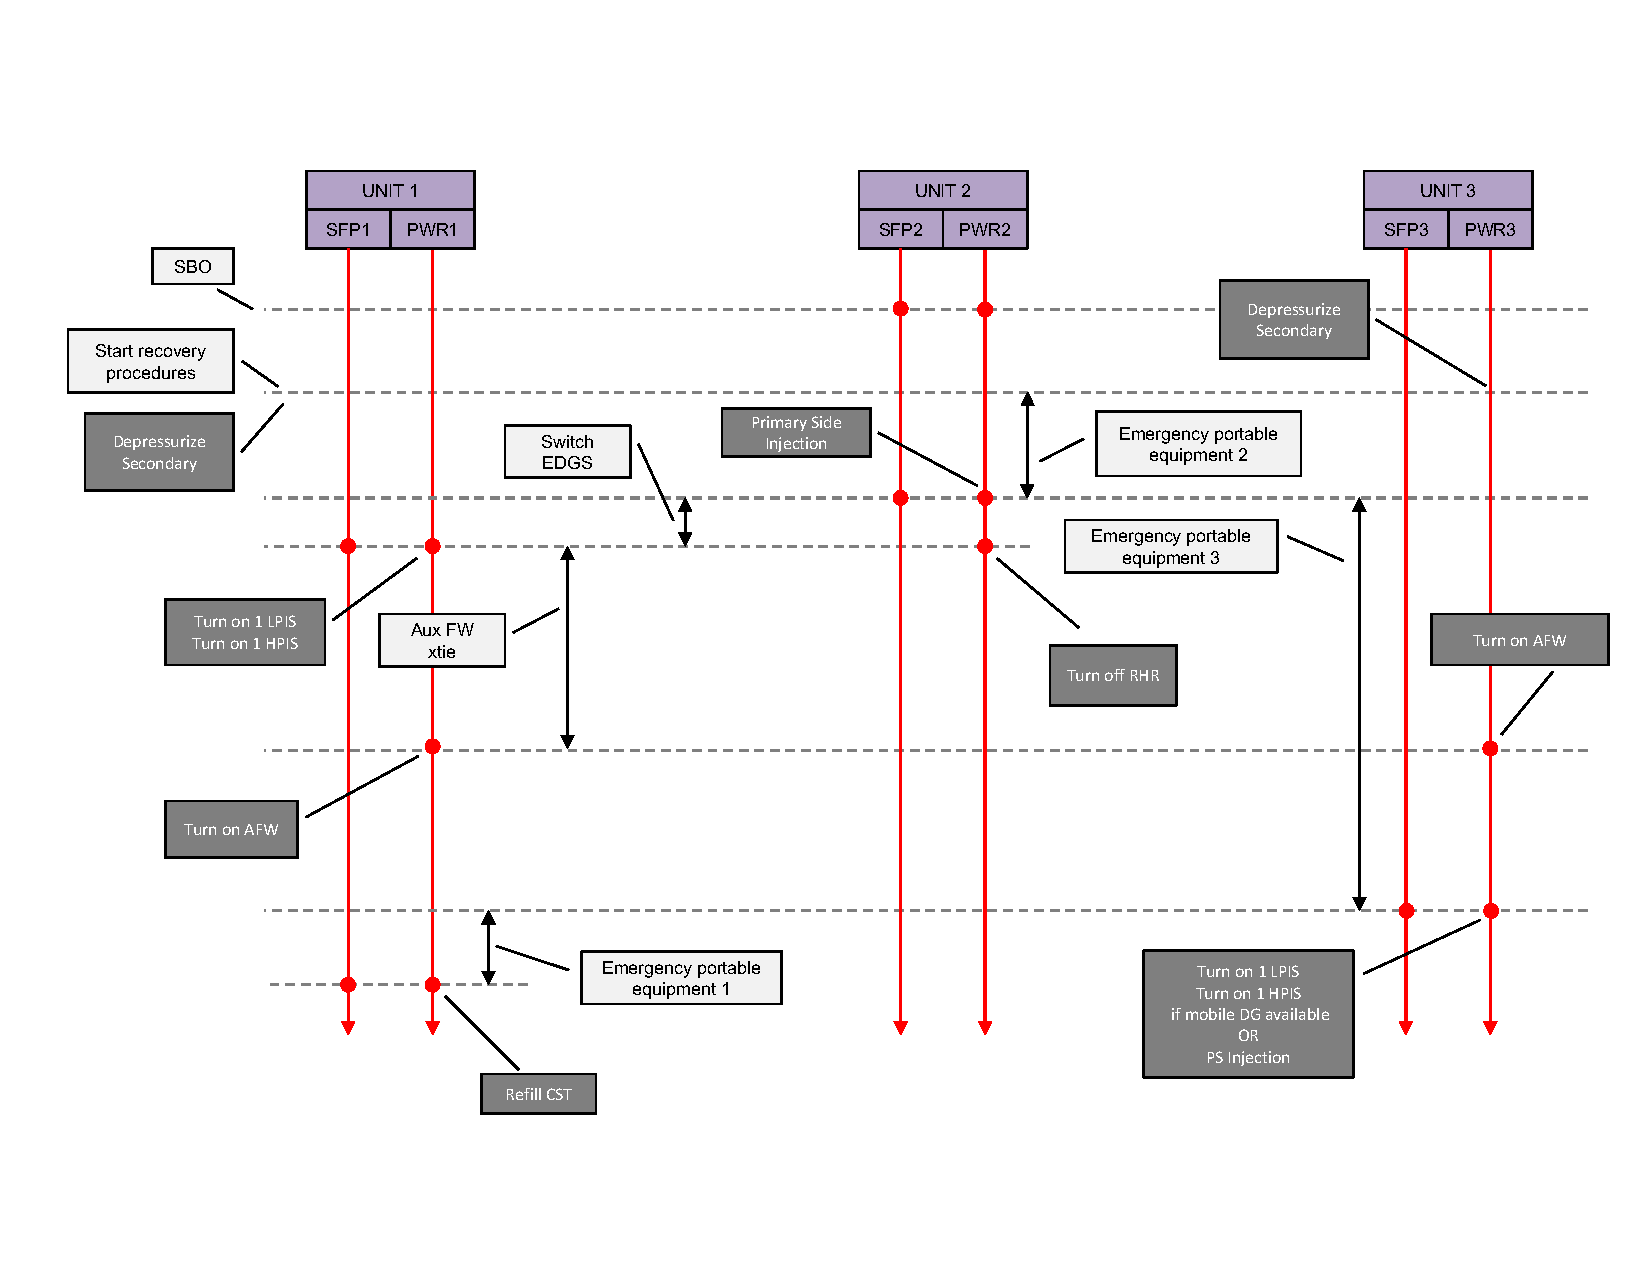
\includegraphics[scale=0.6]{strategy1.pdf}}
    \caption{Sequence of events of recovery strategy 1}
    \label{fig:strategy1Scheme}
\end{figure}

\subsubsection{Strategy 2}
\label{sec:strategy2}

This strategy, similarly to Strategy 1, prioritizes Unit 2 since it is in mid-loop condition; thus, the EPE 
team is initially directed toward this unit. 
Once this task has been accomplished, Unit 3 becomes again now the priority. In order to put this unit in a safe 
condition two parallel directions are followed:

\begin{itemize}
  \item Move the EPE team toward Unit 3 
  \item Align the EDGS from Unit 2 to Unit 1 so that also Unit 1 can be place in a safe condition and provide 
        CST inventory from PWR 2 and PWR 3 (once completed). Note that the CST cross-tie does not provide cooling 
        to the SFP
\end{itemize}

Finally, once Unit 3 EPE has been connected, the EPE team move Unit 1 as indicated also for Strategy 1.

A temporal scheme of the temporal evolution of this accident scenario is shown in Fig.~\ref{fig:strategy2Scheme}.  

\begin{figure}
    \centering
    \centerline{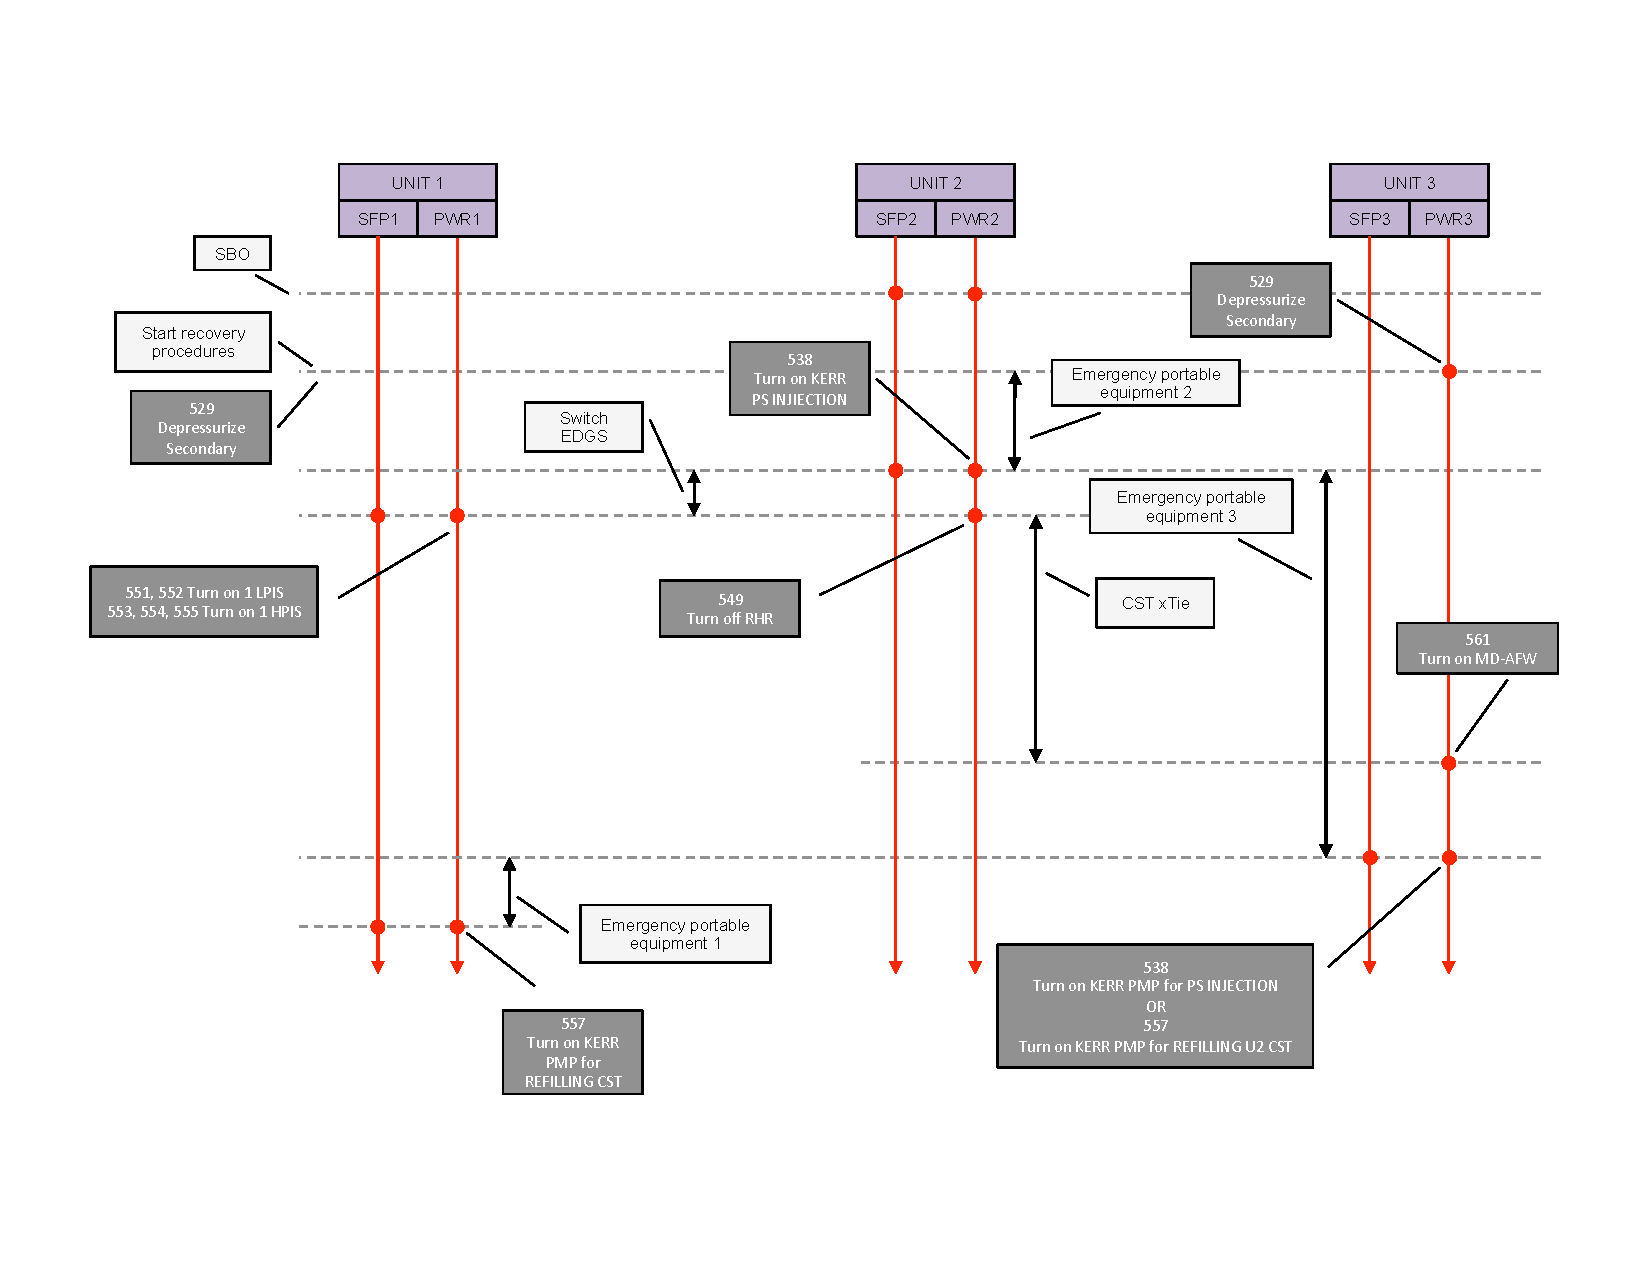
\includegraphics[scale=0.6]{strategy2.pdf}}
    \caption{Sequence of events of recovery strategy 2}
    \label{fig:strategy2Scheme}
\end{figure}

\subsubsection{Strategy 3}
\label{sec:strategy3}

This strategy prioritizes Unit 3; hence the EPE team is initially directed toward this unit. 
Once this task has been accomplished, Unit 1 becomes now the priority. In order to put this unit in a safe 
condition two parallel directions are followed: 

\begin{itemize}
  \item Move the EPE team toward Unit 1 
  \item Perform an AC cross-tie so that AC power generated by EDGS can be employed to provide power to both Unit
        1 and Unit 2. Note that it is here assumed that a correct AC management is implemented in order to avoid
        over-load of the EDGS.
\end{itemize}

Finally, once Unit 1 EPE has been connected, the EPE team move Unit 2. At this point Unit 2 should be already in a 
safe condition since EDGS is still aligned to Unit 2, again, this step has been added since the simulation run (for 
both PWR and SFP) stops when the EPE connected to the unit.

A temporal scheme of the temporal evolution of this accident scenario is shown in Fig.~\ref{fig:strategy3Scheme}

\begin{figure}
    \centering
    \centerline{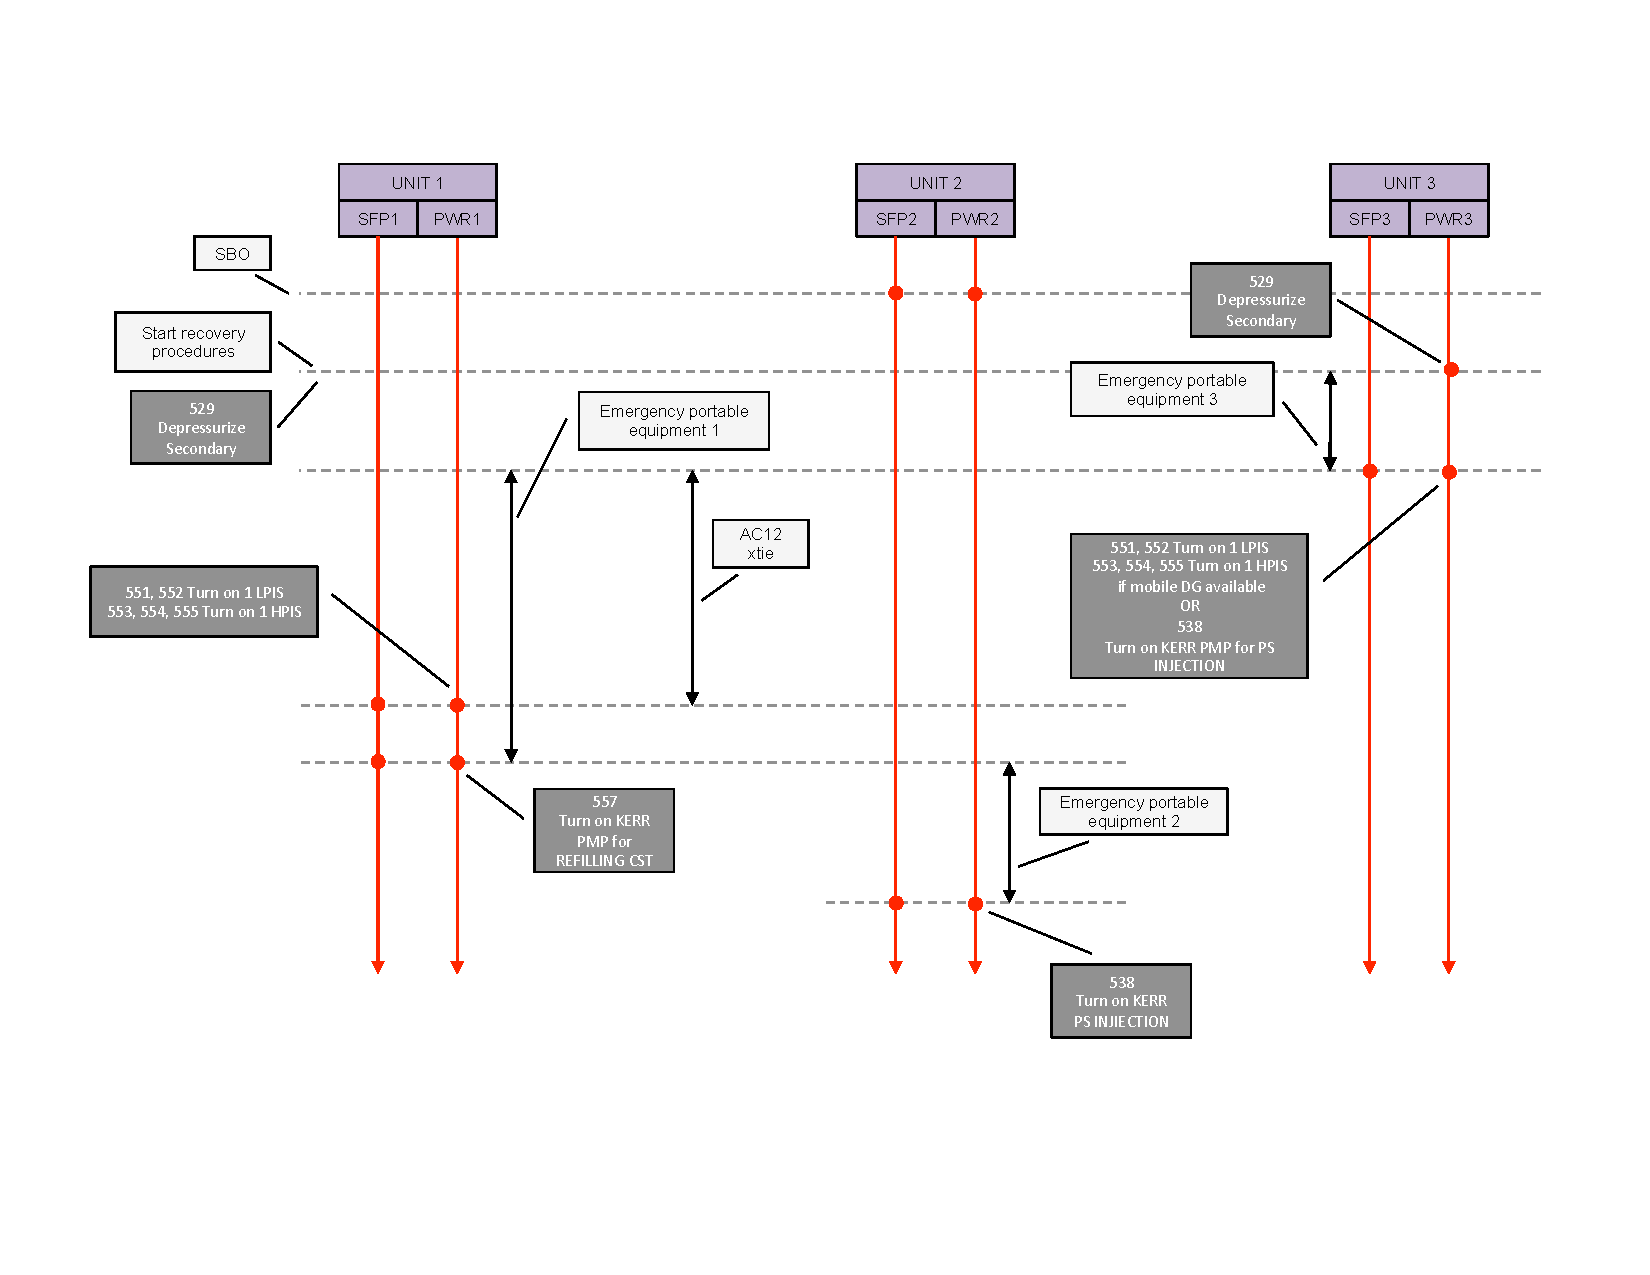
\includegraphics[scale=0.6]{strategy3.pdf}}
    \caption{Sequence of events of recovery strategy 3}
    \label{fig:strategy3Scheme}
\end{figure}

\subsubsection{EDGS involuntary alignment}
\label{sec:EDGSinvolAlign}

As part of the simulation we have introduced a stochastic event: the involuntary alignment of the EDGS.
This event can occur anytime during the simulation and it represents the involuntary alignment of the EDGS 
(initially aligned to Unit 2) to Unit 1. 
While this event can be considered an error of commission from an HRA perspective, from an operational point of view 
it does leave Unit 2 in an unsafe situation but it provide a safe condition to Unit 1. 

Note that now this stochastic element add an additional degree of freedom in the accident progression since the 
occurrence of this event changes the prioritization of the next unit to have the EPE connected.

As an example, Fig.~\ref{fig:strategy3SchemeInvolAlign} shows a possible sequence of events if Strategy 3 
(refer to Section~\ref{sec:strategy3}) has been chosen but with the involuntary alignment of EDGS while the EPE team
is working on Unit 3. Given the unexpected event, the EPE team moves to Unit 2 instead of Unit 1 since Unit 2
has higher priority. The difference sequence of events caused by involuntary alignment of EDGS can be viewed
by comparing Fig.~\ref{fig:strategy3Scheme} with Fig.~\ref{fig:strategy3SchemeInvolAlign}.

\begin{figure}
  \centering
  \centerline{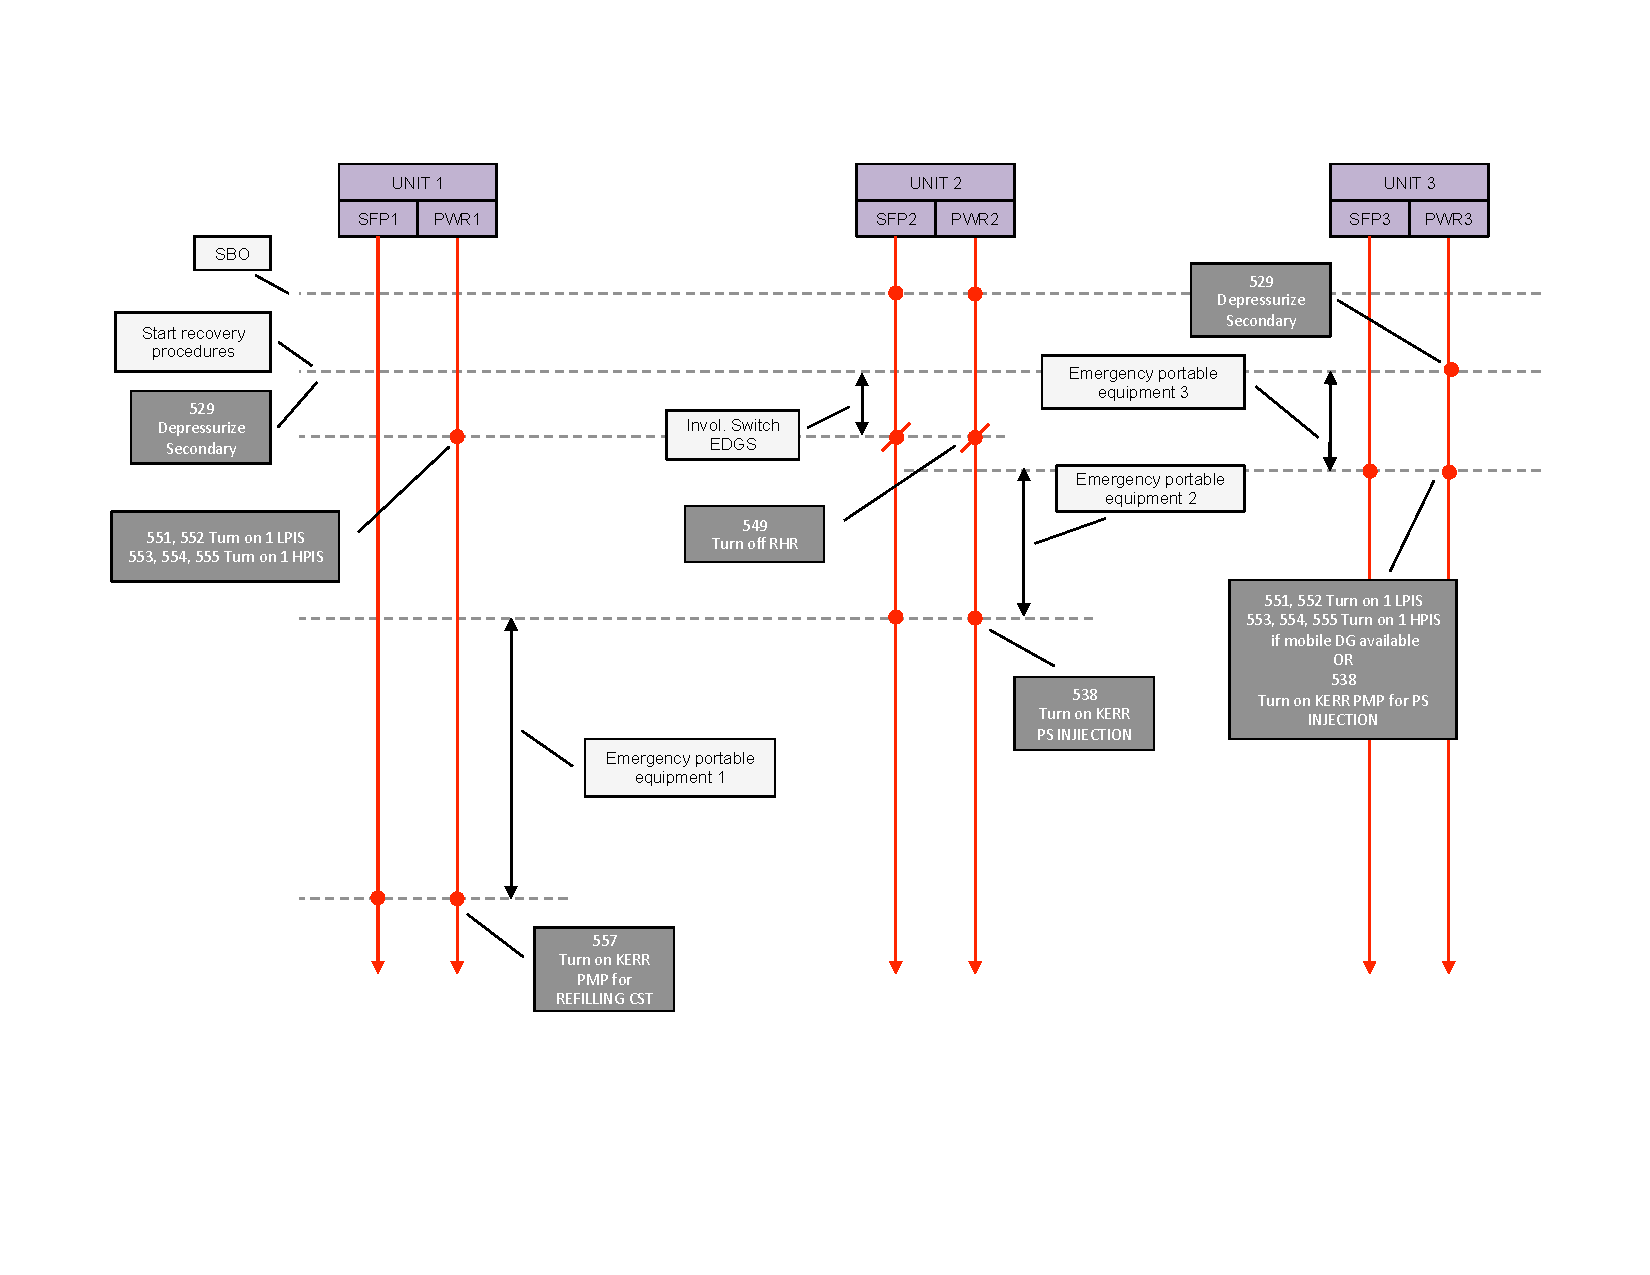
\includegraphics[scale=0.6]{strategy3InvolAlign.pdf}}
  \caption{Sequence of events of recovery strategy 3 with involuntary alignment of EDGS}
  \label{fig:strategy3SchemeInvolAlign}
\end{figure}

\subsection{EPE actions}
\label{sec:EPEactions}

Depending on the unit status different actions can be employed when connecting EPEs to their respective unit.
A summary of the EPE actions for each unit is summarized in Table~\ref{tab:EPEactions}. Note that we have given 

\begin{table}
  \begin{tabular}{|c|l|l|p{5cm}|}
     \hline
       \textbf{Strategy} &  \textbf{PWR1}       &  \textbf{PWR2}         &  \textbf{PWR3}    \\ 
       \hline \hline                                                              
       1        & Refill CST & PS injection & Provide AC power and employ 1 LPIS and 1 HPIS or perform PS injection  \\ \hline
       2        & Refill CST & PS injection & Perform PS injection or refill CST                                     \\ \hline
       3        & Refill CST & PS injection & Provide AC power and employ 1 LPIS and 1 HPIS or perform PS injection  \\ \hline
  \end{tabular}
  \caption{EPE actions for each unit and for each recovery strategy}
  \label{tab:EPEactions}
\end{table} 

